\section{Collection Results}\label{sec:dns_results} % TODO Better section name?

Using the implementation outlined in the previous section, we ran four batches of data collection. This section provides an overview of the results of that collection, including issues we encountered and potential future mitigations for these issues.

\subsection{Server Reliability Filtering}

After filtering authoritative and recursive \dns servers for testing reliability (max coefficient of variation in repeated tests = 0.75), we were left with 387 authoritative servers across 50 states and the District of Columbia and 654 recursive servers across 49 states and the District of Columbia. We could not locate an open recursive \dns server, even unreliable, in the state of Rhode Island. \Cref{fig:dns_cache_manipulation_map_of_authoritative_servers} and \cref{fig:dns_cache_manipulation_map_of_recursive_servers} show the locations of the final server lists for authoritative servers and recursive servers respectively.

\begin{figure}[htb]
    \centering
    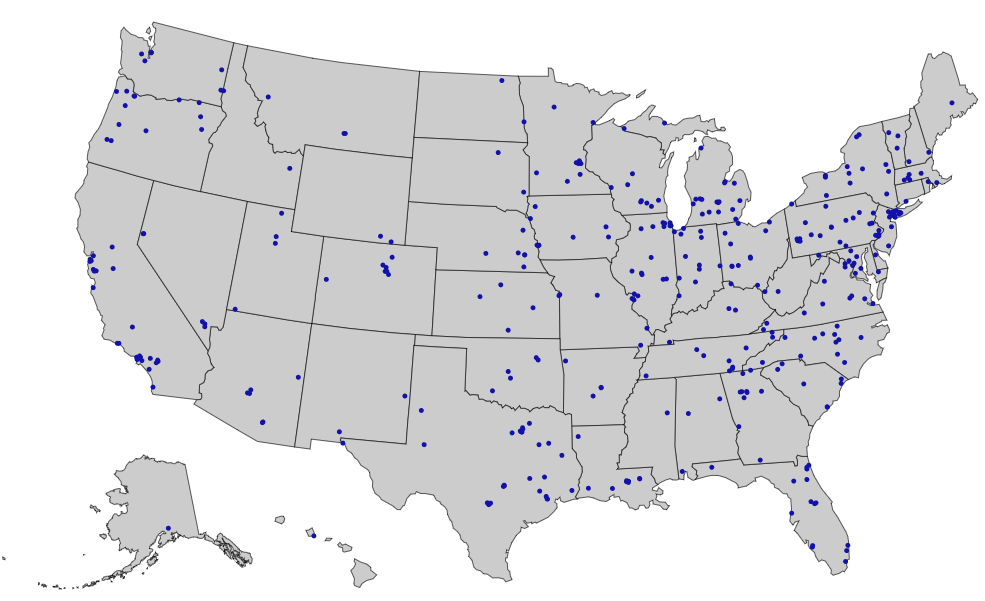
\includegraphics[width=0.75\textwidth]{images/dns/server_locations/auth_server_locations.png}
    \caption{Map of authoritative DNS servers}
    \label{fig:dns_cache_manipulation_map_of_authoritative_servers}
\end{figure}

\begin{figure}[htb]
    \centering
    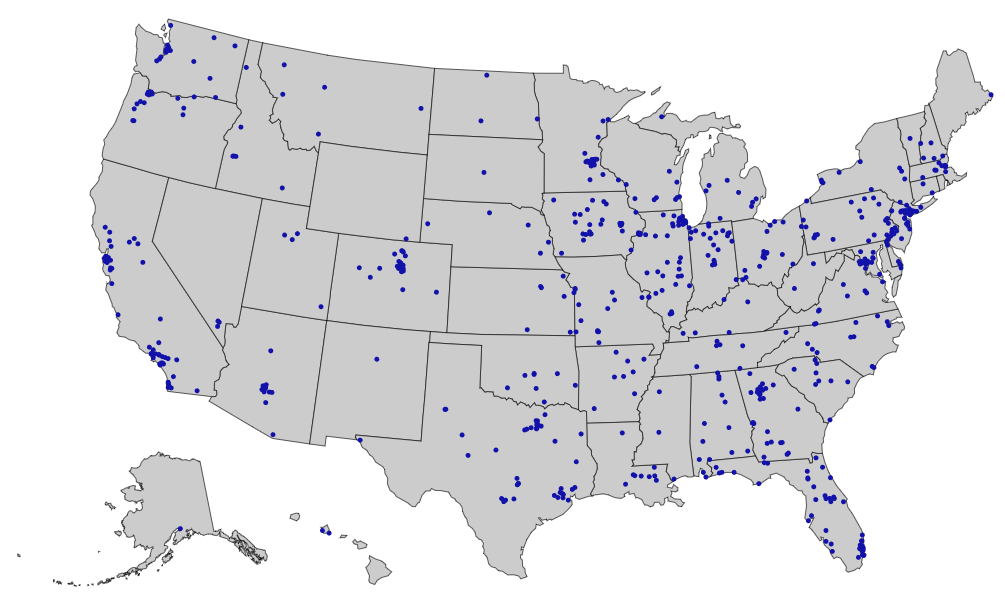
\includegraphics[width=0.75\textwidth]{images/dns/server_locations/rec_server_locations.png}
    \caption{Map of recursive DNS servers}
    \label{fig:dns_cache_manipulation_map_of_recursive_servers}
\end{figure}

\subsection{Data Collection}

Data collection was done in two main batches, along with two supplemental ones to add additional servers and increase geographical coverage. All runs used \texttt{cnn.com} as the domain used to confirm candidate server's status as recursive servers and to test the recursive server's reliability.

\begin{table}[htb]
    \centering
    \begin{tabular}{p{1cm}||p{2cm}|p{2cm}|p{2cm}|p{2cm}|p{4cm} }
    %  \multicolumn{6}{c}{\textbf{Batch Overview}} \\
    %  \hline
     \textbf{\#} & \textbf{Trial Count} & \textbf{Timeout} & \textbf{Records} & \textbf{Runtime} & \textbf{Notes} \\
     \hline
     1 & 5 & 2s & 1,831,495 & 62h & \\
     2 & 10 & 3s & 3,763,311 & 244h & \\
     3 & 10 & 3s & 4,920 & 9m  & Sup. for VT rec. \\
     4 & 10 & 3s & 7,320 & 11m & Sup. for HI auth. \\
     \hline
     \multicolumn{3}{r|}{\textbf{Total}} & 5,607,046 & 306 hours & \\
    \end{tabular}
    \caption{Overview of DNS batch runs}
    \label{tab:dns_batch_overview}
\end{table}

Again, as \cref{tab:dns_batch_overview} shows, the vast majority of data was collected over the course of two collection runs, \#1 and \#2. The first run only conducted five trials for each authoritative-recursive server pair and limited the timeout to for each \texttt{dig} command to two seconds, whereas subsequent runs ran with ten trials and a three second timeout. There are two reasons for this. First, the initial batch was run on \texttt{ccc.wpi.edu}, which has more limitations than the machine used for subsequent runs, \texttt{rambo.wpi.edu}. Additionally, that run was the first major step up from the more limited development test runs and we wanted to minimize time lost in the event something went wrong. On subsequent tests, we had more confidence in the collection scripts and were able to let it run for longer unsupervised.

Batch \#3 was run with a limited number of recursive servers located only in Vermont (with the full authoritative server list) while batch \#4 ran with a limited number of authoritative servers located only in Hawaii (with the full recursive server list). These were run after we discovered that we lacked data of the given type for these states. 

We ran into one issue with batch \#4: the collection scripts randomize the order of all pairs under test to minimize the repetitive requests to the same \dns servers in too short of a time period. However, in both supplemental tests, there were only small numbers of recursive servers (for \#3) or authoritative servers (for \#4). In batch \#4, this resulted in repetitive requests to the same authoritative server in a short period of time, which in turn caused WPI's IT system to believe we were using a \dns tunnel. The use of such a tunnel is prohibited under WPI's Acceptable Use Policy and resulted in a temporary suspension of network privileges.
